\chapter{Batch Size, Dropout and Learning Rate Comparison Data}\label{ch:appBlabel}

\section{Batch Size Test}
\subsubsection{Final table results}
%-------------------------------------------------------
\begin{table}[H]
\begin{minipage}{0.5\textwidth}
\centering
	\caption{Test error rate results.}
	\begin{tabular}{| l | c | c | c |}
	\hline
	Tests & Value & Epoch & Duration \\
	\hline
	Test1 -\tikzcircle[orange, fill=orange]{3pt}- &
	0.1308 & 25.00 & 0s\\
	\hline
	Test2 -\tikzcircle[blue, fill=blue]{3pt}- &
	0.000 & 25.00 & 0s\\
	\hline
	Test5 -\tikzcircle[pink, fill=pink]{3pt}- &
	0.000 & 25.00 & 0s\\
	\hline
	\end{tabular}
\end{minipage}
\begin{minipage}[c]{0.5\textwidth}
\centering
	\caption{Training error rate results.}
	\begin{tabular}{| l | c | c | c |}
	\hline
	Tests & Value & Epoch & Duration \\
	\hline
	Test1 -\tikzcircle[orange, fill=orange]{3pt}- &
	0.1148 & 24.00 & 1h 26m 13s\\
	\hline
	Test2 -\tikzcircle[blue, fill=blue]{3pt}- &
	9.5073e-4 & 24.00 & 18m 50s\\
	\hline
	Test5 -\tikzcircle[pink, fill=pink]{3pt}- &
	5.1858e-4 & 24.00 & 14m 50s\\
	\hline
	\end{tabular}
\end{minipage}%
\end{table}
\begin{table}[H]
\begin{minipage}{0.52\textwidth}
\centering
	\caption{Validation error rate results.}
	\begin{tabular}{| l | c | c | c |}
	\hline
	Tests & Value & Epoch & Duration \\
	\hline
	Test1 -\tikzcircle[orange, fill=orange]{3pt}- &
	0.1608 & 23.00 & 1h 15m 58s\\
	\hline
	Test2 -\tikzcircle[blue, fill=blue]{3pt}- &
	0.05887 & 23.00 & 17m 21s\\
	\hline
	Test5 -\tikzcircle[pink, fill=pink]{3pt}- &
	0.05418 & 23.00 & 13m 50s\\
	\hline
	\end{tabular}
\end{minipage}
\begin{minipage}[c]{0.5\textwidth}
\centering
	\caption{Training average loss results.}
	\begin{tabular}{| l | c | c | c |}
	\hline
	Tests & Value & Epoch & Duration \\
	\hline
	Test1 -\tikzcircle[orange, fill=orange]{3pt}- &
	1.639 & 24.00 & 1h 26m 13s\\
	\hline
	Test2 -\tikzcircle[blue, fill=blue]{3pt}- &
	0.06023 & 24.00 & 18m 50s\\
	\hline
	Test5 -\tikzcircle[pink, fill=pink]{3pt}- &
	0.01988 & 24.00 & 14m 50s\\
	\hline
	\end{tabular}
\end{minipage}%
\end{table}
\begin{figure}[H]
    \centering
    \begin{minipage}{0.5\textwidth}
        \centering
\includegraphics[width=2.5\textwidth, angle=90]		
	{machine_learning/graph_tests/batch_test/test_error_rate}
        \caption{Test error rate.}
    \end{minipage}\hfill
    \begin{minipage}{0.5\textwidth}
        \centering
\includegraphics[width=2.5\textwidth, angle=90]	
	{machine_learning/graph_tests/batch_test/train_error_rate}
        \caption{Training error rate.}
    \end{minipage}
\end{figure}
\begin{figure}[H]
    \centering
    \begin{minipage}{0.5\textwidth}
        \centering
	\includegraphics[width=2.5\textwidth, angle=90]		
	{machine_learning/graph_tests/batch_test/validation_error_rate}
        \caption{Validation error rate.}
    \end{minipage}\hfill
    \begin{minipage}{0.5\textwidth}
        \centering
\includegraphics[width=2.5\textwidth, angle=90]		
	{machine_learning/graph_tests/batch_test/train_avg_loss}
        \caption{Training average loss.}
    \end{minipage}
\end{figure}

%%test error rate
%\begin{figure}[H]
%\centering
%	\includegraphics[width=\textwidth]		
%	{machine_learning/graph_tests/batch_test/test_error_rate}
%	\caption{Test error rate.}
%\end{figure}
%%training error rate
%\begin{figure}[H]
%	\centering
%	\includegraphics[width=\textwidth]		
%	{machine_learning/graph_tests/batch_test/train_error_rate}
%	\caption{Training error rate.}
%\end{figure}
%%validation error rate
%\begin{figure}[H]
%	\centering
%	\includegraphics[width=\textwidth]		
%	{machine_learning/graph_tests/batch_test/validation_error_rate}
%	\caption{Validation error rate.}
%\end{figure}
%%training average loss
%\begin{figure}[H]
%	\centering
%	\includegraphics[width=\textwidth]		
%	{machine_learning/graph_tests/batch_test/train_avg_loss}
%	\caption{Training average loss.}
%\end{figure}
%\begin{table}[H]
%\centering
%	\caption{Test error rate results.}
%	\begin{tabular}{| l | c | c | c |}
%	\hline
%	Tests & Value & Epoch & Duration \\
%	\hline
%	Test1 -\tikzcircle[orange, fill=orange]{3pt}- &
%	0.1308 & 25.00 & 0s\\
%	\hline
%	Test2 -\tikzcircle[blue, fill=blue]{3pt}- &
%	0.000 & 25.00 & 0s\\
%	\hline
%	Test5 -\tikzcircle[pink, fill=pink]{3pt}- &
%	0.000 & 25.00 & 0s\\
%	\hline
%	\end{tabular}
%\end{table}
%\begin{table}[H]
%\centering
%	\caption{Training error rate results.}
%	\begin{tabular}{| l | c | c | c |}
%	\hline
%	Tests & Value & Epoch & Duration \\
%	\hline
%	Test1 -\tikzcircle[orange, fill=orange]{3pt}- &
%	0.1148 & 24.00 & 1h 26m 13s\\
%	\hline
%	Test2 -\tikzcircle[blue, fill=blue]{3pt}- &
%	9.5073e-4 & 24.00 & 18m 50s\\
%	\hline
%	Test5 -\tikzcircle[pink, fill=pink]{3pt}- &
%	5.1858e-4 & 24.00 & 14m 50s\\
%	\hline
%	\end{tabular}
%\end{table}
%\begin{table}[H]
%\centering
%	\caption{Validation error rate results.}
%	\begin{tabular}{| l | c | c | c |}
%	\hline
%	Tests & Value & Epoch & Duration \\
%	\hline
%	Test1 -\tikzcircle[orange, fill=orange]{3pt}- &
%	0.1608 & 23.00 & 1h 15m 58s\\
%	\hline
%	Test2 -\tikzcircle[blue, fill=blue]{3pt}- &
%	0.05887 & 23.00 & 17m 21s\\
%	\hline
%	Test5 -\tikzcircle[pink, fill=pink]{3pt}- &
%	0.05418 & 23.00 & 13m 50s\\
%	\hline
%	\end{tabular}
%\end{table}
%\begin{table}[H]
%\centering
%	\caption{Training average loss results.}
%	\begin{tabular}{| l | c | c | c |}
%	\hline
%	Tests & Value & Epoch & Duration \\
%	\hline
%	Test1 -\tikzcircle[orange, fill=orange]{3pt}- &
%	1.639 & 24.00 & 1h 26m 13s\\
%	\hline
%	Test2 -\tikzcircle[blue, fill=blue]{3pt}- &
%	0.06023 & 24.00 & 18m 50s\\
%	\hline
%	Test5 -\tikzcircle[pink, fill=pink]{3pt}- &
%	0.01988 & 24.00 & 14m 50s\\
%	\hline
%	\end{tabular}
%\end{table}	
%-------------------------------------------------------
\section{Dropout Test}
\subsubsection{Final table results}
\begin{table}[H]
\begin{minipage}{0.5\textwidth}
\centering
	\caption{Test error rate results.}
	\begin{tabular}{| l | c | c | c |}
	\hline
	Tests & Value & Epoch & Duration \\
	\hline
	Test2 -\tikzcircle[blue, fill=blue]{3pt}- &
	0.000 & 25.00 & 0s\\
	\hline
	Test3 -\tikzcircle[red, fill=red]{3pt}- &
	0.030 & 25.00 & 0s\\
	\hline
	Test4 -\tikzcircle[lightblue, fill=lightblue]{3pt}- &
	0.020 & 25.00 & 0s\\
	\hline
	\end{tabular}
\end{minipage}
\begin{minipage}[c]{0.5\textwidth}
\centering
\caption{Training error rate results.}
	\begin{tabular}{| l | c | c | c |}
	\hline
	Tests & Value & Epoch & Duration \\
	\hline
	Test2 -\tikzcircle[blue, fill=blue]{3pt}- &
	9.5973e-4 & 24.00 & 18m 50s\\
	\hline
	Test3 -\tikzcircle[red, fill=red]{3pt}- &
	0.000 & 24.00 & 18m 5s\\
	\hline
	Test4 -\tikzcircle[lightblue, fill=lightblue]{3pt}- &
	6.3331e-3 & 24.00 & 18m 10s\\
	\hline
	\end{tabular}
\end{minipage}%
\end{table}
\begin{table}[H]
\begin{minipage}{0.52\textwidth}
\centering
	\caption{Validation error rate results.}
	\begin{tabular}{| l | c | c | c |}
	\hline
	Tests & Value & Epoch & Duration \\
	\hline
	Test2 -\tikzcircle[blue, fill=blue]{3pt}- &
	0.05887 & 23.00 & 17m 21s\\
	\hline
	Test3 -\tikzcircle[red, fill=red]{3pt}- &
	0.05161 & 23.00 & 16m 36s\\
	\hline
	Test4 -\tikzcircle[lightblue, fill=lightblue]{3pt}- &
	0.02366 & 23.00 & 16m 35s\\
	\hline
	\end{tabular}
\end{minipage}
\begin{minipage}[c]{0.5\textwidth}
\centering
	\caption{Training average loss results.}
	\begin{tabular}{| l | c | c | c |}
	\hline
	Tests & Value & Epoch & Duration \\
	\hline
	Test2 -\tikzcircle[blue, fill=blue]{3pt}- &
	0.06023 & 24.00 & 18m 50s\\
	\hline
	Test3 -\tikzcircle[red, fill=red]{3pt}- &
	3.5483e-4 & 24.00 & 18m 5s\\
	\hline
	Test4 -\tikzcircle[lightblue, fill=lightblue]{3pt}- &
	0.09217 & 24.00 & 18m 10s\\
	\hline
	\end{tabular}
\end{minipage}%
\end{table}
\begin{figure}[H]
    \centering
    \begin{minipage}{0.5\textwidth}
        \centering
\includegraphics[width=2.5\textwidth, angle=90]		
	{machine_learning/graph_tests/dropout_test/test_error_rate}
        \caption{Test error rate.}
    \end{minipage}\hfill
    \begin{minipage}{0.5\textwidth}
        \centering
\includegraphics[width=2.5\textwidth, angle=90]	
	{machine_learning/graph_tests/dropout_test/train_error_rate}
        \caption{Training error rate.}
    \end{minipage}
\end{figure}
\begin{figure}[H]

    \centering
    \begin{minipage}{0.5\textwidth}
        \centering
	\includegraphics[width=2.5\textwidth, angle=90]		
	{machine_learning/graph_tests/dropout_test/validation_error_rate}
        \caption{Validation error rate.}
    \end{minipage}\hfill
    \begin{minipage}{0.5\textwidth}
        \centering
\includegraphics[width=2.5\textwidth, angle=90]		
	{machine_learning/graph_tests/dropout_test/train_avg_loss}
        \caption{Training average loss.}
    \end{minipage}
\end{figure}
%%test error rate
%\begin{figure}[H]
%	\centering
%	\includegraphics[width=\textwidth]		
%	{machine_learning/graph_tests/dropout_test/test_error_rate}
%	\caption{Test error rate.}
%\end{figure}
%%training error rate
%\begin{figure}[H]
%	\centering
%	\includegraphics[width=\textwidth]		
%	{machine_learning/graph_tests/dropout_test/train_error_rate}
%	\caption{Training error rate.}
%\end{figure}	
%%validation error rate
%\begin{figure}[H]
%	\centering
%	\includegraphics[width=\textwidth]		
%	{machine_learning/graph_tests/dropout_test/validation_error_rate}
%	\caption{Validation error rate.}
%\end{figure}
%%training avarage loss
%\begin{figure}[H]
%	\centering
%	\includegraphics[width=\textwidth]		
%	{machine_learning/graph_tests/dropout_test/train_avg_loss}
%	\caption{Training average loss.}
%\end{figure}	%-----------------------------------------------------
%\begin{table}[H]
%\centering
%	\caption{Test error rate results.}
%	\begin{tabular}{| l | c | c | c |}
%	\hline
%	Tests & Value & Epoch & Duration \\
%	\hline
%	Test2 -\tikzcircle[blue, fill=blue]{3pt}- &
%	0.000 & 25.00 & 0s\\
%	\hline
%	Test3 -\tikzcircle[red, fill=red]{3pt}- &
%	0.030 & 25.00 & 0s\\
%	\hline
%	Test4 -\tikzcircle[lightblue, fill=lightblue]{3pt}- &
%	0.020 & 25.00 & 0s\\
%	\hline
%	\end{tabular}
%\end{table}	
%\begin{table}[H]
%\centering
%	\caption{Training error rate results.}
%	\begin{tabular}{| l | c | c | c |}
%	\hline
%	Tests & Value & Epoch & Duration \\
%	\hline
%	Test2 -\tikzcircle[blue, fill=blue]{3pt}- &
%	9.5973e-4 & 24.00 & 18m 50s\\
%	\hline
%	Test3 -\tikzcircle[red, fill=red]{3pt}- &
%	0.000 & 24.00 & 18m 5s\\
%	\hline
%	Test4 -\tikzcircle[lightblue, fill=lightblue]{3pt}- &
%	6.3331e-3 & 24.00 & 18m 10s\\
%	\hline
%	\end{tabular}
%\end{table}	
%\begin{table}[H]
%\centering
%	\caption{Validation error rate results.}
%	\begin{tabular}{| l | c | c | c |}
%	\hline
%	Tests & Value & Epoch & Duration \\
%	\hline
%	Test2 -\tikzcircle[blue, fill=blue]{3pt}- &
%	0.05887 & 23.00 & 17m 21s\\
%	\hline
%	Test3 -\tikzcircle[red, fill=red]{3pt}- &
%	0.05161 & 23.00 & 16m 36s\\
%	\hline
%	Test4 -\tikzcircle[lightblue, fill=lightblue]{3pt}- &
%	0.02366 & 23.00 & 16m 35s\\
%	\hline
%	\end{tabular}
%\end{table}	
%\begin{table}[H]
%\centering
%	\caption{Training average loss results.}
%	\begin{tabular}{| l | c | c | c |}
%	\hline
%	Tests & Value & Epoch & Duration \\
%	\hline
%	Test2 -\tikzcircle[blue, fill=blue]{3pt}- &
%	0.06023 & 24.00 & 18m 50s\\
%	\hline
%	Test3 -\tikzcircle[red, fill=red]{3pt}- &
%	3.5483e-4 & 24.00 & 18m 5s\\
%	\hline
%	Test4 -\tikzcircle[lightblue, fill=lightblue]{3pt}- &
%	0.09217 & 24.00 & 18m 10s\\
%	\hline
%	\end{tabular}
%\end{table}	
%-----------------------------------------------------

\section{Learning Rate Test}
\subsubsection{Final table results}
\begin{table}[H]
\begin{minipage}{0.5\textwidth}
\centering
	\caption{Test error rate results.}
	\begin{tabular}{| l | c | c | c |}
	\hline
	Tests & Value & Epoch & Duration \\
	\hline
	Test5 -\tikzcircle[pink, fill=pink]{3pt}- &
	0.000 & 25.00 & 0s\\
	\hline
	Test6 -\tikzcircle[turquoise, fill=turquoise]{3pt}- &
	0.8992 & 25.00 & 0s\\
	\hline
	\end{tabular}
\end{minipage}
\begin{minipage}[c]{0.5\textwidth}
\centering
	\caption{Training error rate results.}
	\begin{tabular}{| l | c | c | c |}
	\hline
	Tests & Value & Epoch & Duration \\
	\hline
	Test5 -\tikzcircle[pink, fill=pink]{3pt}- &
	5.1858e-4 & 24.00 & 14m 50s\\
	\hline
	Test6 -\tikzcircle[turquoise, fill=turquoise]{3pt}- &
	0.9188 & 24.00 & 12m 29s\\
	\hline
	\end{tabular}
\end{minipage}%
\end{table}
\begin{table}[H]
\begin{minipage}{0.52\textwidth}
\centering
	\caption{Validation error rate results.}
	\begin{tabular}{| l | c | c | c |}
	\hline
	Tests & Value & Epoch & Duration \\
	\hline
	Test5 -\tikzcircle[pink, fill=pink]{3pt}- &
	0.02661 & 23.00 & 13m 50s\\
	\hline
	Test6 -\tikzcircle[turquoise, fill=turquoise]{3pt}- &
	1.152 & 23.00 & 11m 29s\\
	\hline
	\end{tabular}
\end{minipage}
\begin{minipage}[c]{0.5\textwidth}
\centering
	\caption{Training average loss results.}
	\begin{tabular}{| l | c | c | c |}
	\hline
	Tests & Value & Epoch & Duration \\
	\hline
	Test5 -\tikzcircle[pink, fill=pink]{3pt}- &
	0.01988 & 24.00 & 14m 50s\\
	\hline
	Test6 -\tikzcircle[turquoise, fill=turquoise]{3pt}- &
	12.56 & 24.00 & 12m 29s\\
	\hline
	\end{tabular}
\end{minipage}%
\end{table}
\begin{figure}[H]
    \centering
    \begin{minipage}{0.5\textwidth}
        \centering
\includegraphics[width=2.5\textwidth, angle=90]		
	{machine_learning/graph_tests/learning_rate_test/test_error_rate}
        \caption{Test error rate.}
    \end{minipage}\hfill
    \begin{minipage}{0.5\textwidth}
        \centering
\includegraphics[width=2.5\textwidth, angle=90]	
	{machine_learning/graph_tests/learning_rate_test/train_error_rate}
        \caption{Training error rate.}
    \end{minipage}
\end{figure}
\begin{figure}[H]
    \centering
    \begin{minipage}{0.5\textwidth}
        \centering
	\includegraphics[width=2.5\textwidth, angle=90]		
	{machine_learning/graph_tests/learning_rate_test/validation_error_rate}
        \caption{Validation error rate.}
    \end{minipage}\hfill
    \begin{minipage}{0.5\textwidth}
        \centering
\includegraphics[width=2.5\textwidth, angle=90]		
	{machine_learning/graph_tests/learning_rate_test/train_avg_loss}
        \caption{Training average loss.}
    \end{minipage}
\end{figure}

%%test error rate
%\begin{figure}[H]
%	\centering
%	\includegraphics[width=\textwidth]		
%	{machine_learning/graph_tests/learning_rate_test/test_error_rate}
%	\caption{Test error rate.}
%\end{figure}
%%training error rate
%\begin{figure}[H]
%	\centering
%	\includegraphics[width=\textwidth]		
%	{machine_learning/graph_tests/learning_rate_test/train_error_rate}
%	\caption{Training error rate.}
%\end{figure}
%%validation error rate
%\begin{figure}[H]
%	\centering
%	\includegraphics[width=\textwidth]		
%	{machine_learning/graph_tests/learning_rate_test/validation_error_rate}
%	\caption{Validation error rate.}
%\end{figure}	
%%training avarage loss
%\begin{figure}[H]
%	\centering
%	\includegraphics[width=\textwidth]		
%	{machine_learning/graph_tests/learning_rate_test/train_avg_loss}
%	\caption{Training average loss.}
%\end{figure}
%\begin{table}[H]
%\centering
%	\caption{Test error rate results.}
%	\begin{tabular}{| l | c | c | c |}
%	\hline
%	Tests & Value & Epoch & Duration \\
%	\hline
%	Test5 -\tikzcircle[pink, fill=pink]{3pt}- &
%	0.000 & 25.00 & 0s\\
%	\hline
%	Test6 -\tikzcircle[turquoise, fill=turquoise]{3pt}- &
%	0.8992 & 25.00 & 0s\\
%	\hline
%	\end{tabular}
%\end{table}	
%\begin{table}[H]
%\centering
%	\caption{Training error rate results.}
%	\begin{tabular}{| l | c | c | c |}
%	\hline
%	Tests & Value & Epoch & Duration \\
%	\hline
%	Test5 -\tikzcircle[pink, fill=pink]{3pt}- &
%	5.1858e-4 & 24.00 & 14m 50s\\
%	\hline
%	Test6 -\tikzcircle[turquoise, fill=turquoise]{3pt}- &
%	0.9188 & 24.00 & 12m 29s\\
%	\hline
%	\end{tabular}
%\end{table}	
%\begin{table}[H]
%\centering
%	\caption{Validation error rate results.}
%	\begin{tabular}{| l | c | c | c |}
%	\hline
%	Tests & Value & Epoch & Duration \\
%	\hline
%	Test5 -\tikzcircle[pink, fill=pink]{3pt}- &
%	0.02661 & 23.00 & 13m 50s\\
%	\hline
%	Test6 -\tikzcircle[turquoise, fill=turquoise]{3pt}- &
%	1.152 & 23.00 & 11m 29s\\
%	\hline
%	\end{tabular}
%\end{table}	
%\begin{table}[H]
%\centering
%	\caption{Training average loss results.}
%	\begin{tabular}{| l | c | c | c |}
%	\hline
%	Tests & Value & Epoch & Duration \\
%	\hline
%	Test5 -\tikzcircle[pink, fill=pink]{3pt}- &
%	0.01988 & 24.00 & 14m 50s\\
%	\hline
%	Test6 -\tikzcircle[turquoise, fill=turquoise]{3pt}- &
%	12.56 & 24.00 & 12m 29s\\
%	\hline
%	\end{tabular}
%\end{table}		
